\documentclass[12pt]{article}

% Core math
\usepackage{amsmath, amssymb, amsthm}

% Diagrams
\usepackage{tikz-cd}
\usepackage{tikz}
\usetikzlibrary{positioning, arrows.meta, decorations.pathmorphing, calc}

% References
\usepackage{hyperref}
\usepackage{cleveref}

% Graphics
\usepackage{graphicx}

% Page layout
\usepackage[margin=1in]{geometry}

% GrokRxiv sidebar
\usepackage{everypage}
\usepackage{xcolor}

% Theorem environments
\newtheorem{theorem}{Theorem}[section]
\newtheorem{proposition}[theorem]{Proposition}
\newtheorem{lemma}[theorem]{Lemma}
\newtheorem{corollary}[theorem]{Corollary}
\theoremstyle{definition}
\newtheorem{definition}[theorem]{Definition}
\theoremstyle{remark}
\newtheorem{remark}[theorem]{Remark}

% Custom commands
\newcommand{\Lagr}{\mathcal{L}}
\newcommand{\Hamil}{\mathcal{H}}
\newcommand{\CPT}{\mathsf{CPT}}
\newcommand{\C}{\mathsf{C}}
\newcommand{\PP}{\mathsf{P}}
\newcommand{\T}{\mathsf{T}}
\newcommand{\CP}{\mathsf{CP}}
\newcommand{\psibar}{\bar{\psi}}
\newcommand{\bra}[1]{\langle #1 |}
\newcommand{\ket}[1]{| #1 \rangle}
\newcommand{\braket}[2]{\langle #1 | #2 \rangle}
\newcommand{\abs}[1]{\left| #1 \right|}
\newcommand{\tr}{\operatorname{tr}}
\newcommand{\diag}{\operatorname{diag}}
\newcommand{\GeV}{\,\text{GeV}}
\newcommand{\MeV}{\,\text{MeV}}
\newcommand{\keV}{\,\text{keV}}

% GrokRxiv DOI Sidebar
\definecolor{grokgray}{RGB}{110,110,110}
\AddEverypageHook{%
  \ifnum\value{page}=1
    \begin{tikzpicture}[remember picture, overlay]
      \node[
        rotate=90,
        anchor=south,
        font=\Large\sffamily\bfseries\color{grokgray},
        inner sep=0pt
      ] at ([xshift=38pt, yshift=0.52\paperheight]current page.south west)
      {GrokRxiv:2026.04.anti-matter\quad
       [\,hep-ph\,]\quad
       14 Apr 2026};
    \end{tikzpicture}
  \fi
}

\title{\textbf{Anti-Matter in the Modular Physics Framework:\\
CPT Symmetry, CP Violation, and Hierarchical Emergence\\
of the Baryon Asymmetry}}
\author{Matthew Long \\
\textit{The YonedaAI Collaboration} \\
\textit{YonedaAI Research Collective} \\
Chicago, IL \\
\texttt{matthew@yonedaai.com} $\cdot$ \url{https://yonedaai.com}}
\date{April 14, 2026}

\begin{document}

\maketitle

\begin{abstract}
We present a comprehensive treatment of anti-matter within the modular physics framework,
in which the laws of physics compose hierarchically: Law~I (Size-Aware) $\to$ Law~II
(Thermal) $\to$ Law~III (Quantum) $\to$ Law~IV (Gravitational). Anti-matter emerges
as a necessary consequence of the modular composition of quantum mechanics with special
relativity at Law~III, through the Dirac equation and its negative-energy solutions.
We provide rigorous derivations of the CPT theorem and its implications for particle--antiparticle
symmetry, develop the CKM matrix formalism and the origin of CP violation from the complex
phase requiring three quark generations, and analyze the Sakharov conditions for baryogenesis.
We show that CP violation creates asymmetry at each compositional level of the modular framework:
at the quantum level through the CKM phase, at the thermal level through departure from equilibrium
during cosmological phase transitions, and at the gravitational frontier through the observed
baryon-to-photon ratio $\eta \approx 6.1 \times 10^{-10}$. Current experimental results from
CERN (ALPHA, BASE, AEgIS) and LHCb (2025 baryon CP violation) are reviewed, along with
applications including positron emission tomography. We identify the insufficiency of
Standard Model CP violation for baryogenesis as a critical open problem pointing toward
physics beyond the Standard Model.
\end{abstract}

\tableofcontents
\newpage

%==============================================================================
\section{Introduction}
\label{sec:introduction}
%==============================================================================

The existence of anti-matter is one of the most profound predictions of twentieth-century
physics. When Paul Dirac sought to reconcile quantum mechanics with Einstein's special
relativity in 1928, his equation for the relativistic electron admitted solutions with
negative energy---solutions that, upon proper reinterpretation, correspond to particles
of identical mass but opposite quantum numbers: antiparticles~\cite{Dirac1928,Dirac1930}.
The experimental confirmation of the positron by Carl Anderson in 1932 (published 1933)~\cite{Anderson1933}
established the reality of anti-matter and opened a domain of inquiry that remains
active nearly a century later.

In this paper, we analyze anti-matter through the lens of the \emph{modular physics
framework}, in which the laws of physics are organized as a hierarchical composition:

\begin{itemize}
    \item \textbf{Law~I (Size-Aware)}: Physical systems are characterized by their
    spatial extent and the relevant length scales. At this level, matter and anti-matter
    are described by their macroscopic properties---mass, charge, and spatial extent.

    \item \textbf{Law~II (Thermal)}: Statistical mechanics governs the behavior of
    large ensembles of particles. The thermal level introduces the concepts of
    equilibrium, entropy, and phase transitions. The baryon-to-photon ratio
    $\eta \approx 6.1 \times 10^{-10}$ is a thermal relic encoding the history of
    matter--antimatter asymmetry generation.

    \item \textbf{Law~III (Quantum)}: Quantum field theory provides the microscopic
    description of particles and their interactions. Anti-matter \emph{emerges} at
    this level as a necessary consequence of composing quantum mechanics with
    Lorentz invariance. The CPT theorem, the Dirac equation, and the CKM mechanism
    of CP violation all reside at this level.

    \item \textbf{Law~IV (Gravitational)}: General relativity and its quantum
    extensions describe the gravitational interaction. Whether antimatter gravitates
    identically to matter is a question at this compositional frontier, recently
    addressed by the ALPHA-g experiment at CERN~\cite{ALPHA2023}.
\end{itemize}

The key insight of the modular framework is that each compositional level produces
\emph{emergent properties} not present at lower levels. Anti-matter is the paradigmatic
example: it is absent from non-relativistic quantum mechanics (Law~III composed only
with Galilean symmetry) but emerges inevitably when quantum mechanics is composed with
Lorentz invariance. Similarly, the matter--antimatter asymmetry is absent from
zero-temperature quantum field theory but emerges when the quantum level is composed
with the thermal level (Law~II) under the Sakharov conditions.

The structure of this paper is as follows. In \cref{sec:dirac}, we derive the Dirac
equation and show how anti-matter arises from its solution structure.
\Cref{sec:cpt} presents the CPT theorem and its proof.
\Cref{sec:cp_violation} develops the CKM matrix formalism and the mechanism of CP violation.
\Cref{sec:baryogenesis} analyzes the matter--antimatter asymmetry problem and the
Sakharov conditions.
\Cref{sec:modular} presents the modular framework interpretation of anti-matter and CP violation.
\Cref{sec:experiments} reviews current experimental results.
\Cref{sec:applications} discusses applications of anti-matter.
\Cref{sec:results} collects the main mathematical results.
\Cref{sec:discussion} discusses implications and open problems.
\Cref{sec:conclusion} concludes.

%==============================================================================
\section{The Dirac Equation and the Prediction of Anti-Matter}
\label{sec:dirac}
%==============================================================================

\subsection{Motivation: Klein--Gordon Equation and Its Deficiencies}

The naive relativistic generalization of the Schr\"odinger equation uses the
energy--momentum relation $E^2 = \mathbf{p}^2 c^2 + m^2 c^4$ with the substitutions
$E \to i\hbar \partial_t$ and $\mathbf{p} \to -i\hbar \nabla$, yielding the
Klein--Gordon equation:
\begin{equation}
\label{eq:klein_gordon}
\left( \frac{1}{c^2}\frac{\partial^2}{\partial t^2} - \nabla^2 + \frac{m^2 c^2}{\hbar^2} \right) \phi = 0.
\end{equation}
In natural units ($\hbar = c = 1$), this becomes $(\partial_\mu \partial^\mu + m^2)\phi = 0$.

The Klein--Gordon equation has two critical problems as a single-particle wave equation:
\begin{enumerate}
    \item The probability density $\rho = \frac{i}{2m}\left(\phi^* \partial_t \phi - \phi \partial_t \phi^*\right)$ is \emph{not positive definite}, since the equation is second-order in time.
    \item The energy eigenvalues $E = \pm\sqrt{\mathbf{p}^2 + m^2}$ include negative values, with no lower bound.
\end{enumerate}

\subsection{Dirac's Derivation}

\begin{definition}[Dirac Equation]
\label{def:dirac_eq}
The Dirac equation is the first-order relativistic wave equation for a spin-$\frac{1}{2}$
fermion of mass $m$:
\begin{equation}
\label{eq:dirac}
(i\gamma^\mu \partial_\mu - m)\psi = 0,
\end{equation}
where $\psi$ is a four-component Dirac spinor and $\gamma^\mu$ ($\mu = 0,1,2,3$) are
$4 \times 4$ matrices satisfying the Clifford algebra
\begin{equation}
\label{eq:clifford}
\{\gamma^\mu, \gamma^\nu\} \equiv \gamma^\mu \gamma^\nu + \gamma^\nu \gamma^\mu = 2g^{\mu\nu} \mathbf{1}_4,
\end{equation}
with $g^{\mu\nu} = \diag(+1,-1,-1,-1)$ the Minkowski metric.
\end{definition}

Dirac's strategy was to find a Hamiltonian \emph{linear} in the spatial derivatives
(and hence first-order in time), ensuring a positive-definite probability density.
Writing $i\partial_t \psi = H_D \psi$ with $H_D = \boldsymbol{\alpha} \cdot \mathbf{p} + \beta m$,
the requirement that $H_D^2 = \mathbf{p}^2 + m^2$ (the relativistic dispersion relation)
imposes:
\begin{equation}
\label{eq:dirac_algebra}
\{\alpha^i, \alpha^j\} = 2\delta^{ij}, \quad \{\alpha^i, \beta\} = 0, \quad \beta^2 = \mathbf{1}.
\end{equation}
These anti-commutation relations cannot be satisfied by ordinary numbers or $2 \times 2$
matrices; the minimum dimension is $4 \times 4$.

\begin{remark}
The connection $\gamma^0 = \beta$ and $\gamma^i = \beta \alpha^i$ relates the Hamiltonian
form to the covariant form~\eqref{eq:dirac}. In the Dirac (standard) representation:
\begin{equation}
\gamma^0 = \begin{pmatrix} \mathbf{1}_2 & 0 \\ 0 & -\mathbf{1}_2 \end{pmatrix}, \quad
\gamma^i = \begin{pmatrix} 0 & \sigma^i \\ -\sigma^i & 0 \end{pmatrix},
\end{equation}
where $\sigma^i$ are the Pauli matrices.
\end{remark}

\subsection{Plane-Wave Solutions and Negative-Energy States}

Seeking plane-wave solutions $\psi(x) = u(\mathbf{p}) e^{-ip \cdot x}$ with
four-momentum $p^\mu = (E, \mathbf{p})$, the Dirac equation becomes
$(\gamma^\mu p_\mu - m)u(\mathbf{p}) = 0$, or equivalently
$(\slashed{p} - m)u = 0$ where $\slashed{p} \equiv \gamma^\mu p_\mu$.

\begin{proposition}[Energy Spectrum of the Dirac Equation]
\label{prop:energy_spectrum}
The Dirac equation admits four linearly independent plane-wave solutions for each
three-momentum $\mathbf{p}$:
\begin{itemize}
    \item Two positive-energy solutions with $E = +E_{\mathbf{p}} \equiv +\sqrt{\mathbf{p}^2 + m^2}$,
    corresponding to spin-up and spin-down states;
    \item Two negative-energy solutions with $E = -E_{\mathbf{p}}$.
\end{itemize}
\end{proposition}

\begin{proof}
The equation $(\slashed{p} - m)u = 0$ has nontrivial solutions when
$\det(\slashed{p} - m) = 0$. Computing:
\begin{equation}
(\slashed{p} - m)(\slashed{p} + m) = \slashed{p}^2 - m^2 = p_\mu p^\mu - m^2 = E^2 - \mathbf{p}^2 - m^2.
\end{equation}
This vanishes when $E^2 = \mathbf{p}^2 + m^2$, giving $E = \pm E_{\mathbf{p}}$.
For each sign of energy, the rank of $(\slashed{p} - m)$ is 2 (the $4 \times 4$
matrix has two-dimensional null space), yielding two independent spinor solutions
corresponding to the two spin orientations.
\end{proof}

\subsection{Feynman--St\"uckelberg Interpretation}

The negative-energy solutions posed a crisis: an electron could radiate photons and
cascade to arbitrarily negative energies. Dirac's initial resolution was the
\emph{Dirac sea}: all negative-energy states are filled (by the Pauli exclusion principle
for fermions), and a ``hole'' in this sea behaves as a positive-energy, positively-charged
particle---the positron.

The modern interpretation, due to Feynman and St\"uckelberg, is more elegant:

\begin{definition}[Feynman--St\"uckelberg Interpretation]
A negative-energy solution propagating backward in time is equivalent to a
positive-energy antiparticle propagating forward in time. Formally, the
negative-energy solution
\begin{equation}
\psi_{\text{neg}}(x) = v(\mathbf{p}) e^{+i p \cdot x} \quad \text{with } p^0 = E_{\mathbf{p}} > 0
\end{equation}
describes an antiparticle (positron) with momentum $\mathbf{p}$, energy $+E_{\mathbf{p}}$,
and opposite quantum numbers (charge $+e$).
\end{definition}

\begin{theorem}[Emergent Anti-Matter from Modular Composition]
\label{thm:emergent_antimatter}
The existence of antiparticles is a necessary consequence of composing quantum
mechanics (unitarity, superposition) with special relativity (Lorentz invariance,
$E^2 = p^2 + m^2$). No consistent relativistic quantum theory of a single species
of charged particle exists.
\end{theorem}

\begin{proof}[Proof sketch]
We argue by contradiction. Suppose a relativistic quantum theory describes only
particles (no antiparticles). Then:
\begin{enumerate}
    \item Lorentz invariance requires the dispersion relation $E^2 = p^2 + m^2$.
    \item Quantum mechanics requires that the time evolution be generated by a
    Hamiltonian, and the spectrum must be bounded below for stability.
    \item The Dirac equation (the unique first-order Lorentz-covariant equation for
    spin-$\frac{1}{2}$) necessarily has both $E > 0$ and $E < 0$ solutions
    (Proposition~\ref{prop:energy_spectrum}).
    \item Restricting to positive-energy solutions alone is not Lorentz-invariant:
    a Lorentz boost can mix positive and negative frequencies~\cite{Weinberg1995}.
    \item Therefore, consistency requires including the negative-energy solutions,
    interpreted as antiparticles via the Feynman--St\"uckelberg prescription.
\end{enumerate}
In quantum field theory, this is made precise: the Dirac field operator
$\hat{\psi}(x) = \sum_s \int \frac{d^3p}{(2\pi)^3 2E_\mathbf{p}} \left[
\hat{a}_s(\mathbf{p}) u_s(\mathbf{p}) e^{-ip\cdot x} +
\hat{b}_s^\dagger(\mathbf{p}) v_s(\mathbf{p}) e^{+ip\cdot x} \right]$
necessarily contains both particle annihilation operators $\hat{a}_s$ and
antiparticle creation operators $\hat{b}_s^\dagger$. Causality (microcausality
condition $\{\hat{\psi}(x), \hat{\psi}^\dagger(y)\} = 0$ for spacelike
$(x-y)^2 < 0$) requires both terms.
\end{proof}

This is the central example of emergence in the modular framework: the composition
of Law~III (Quantum) with Lorentz symmetry produces anti-matter as an emergent
phenomenon that is absent from either ingredient alone.

%==============================================================================
\section{CPT Symmetry and Its Proof}
\label{sec:cpt}
%==============================================================================

\subsection{The Discrete Symmetries C, P, and T}

\begin{definition}[Charge Conjugation $\C$]
\label{def:charge_conj}
Charge conjugation $\C$ transforms a particle into its antiparticle while preserving
spacetime coordinates:
\begin{equation}
\C \psi(x) \C^{-1} = \eta_C C \psibar^T(x),
\end{equation}
where $C = i\gamma^2 \gamma^0$ is the charge conjugation matrix satisfying
$C \gamma^\mu C^{-1} = -(\gamma^\mu)^T$, and $\eta_C$ is a phase factor
($|\eta_C| = 1$).
\end{definition}

\begin{definition}[Parity $\PP$]
\label{def:parity}
Parity $\PP$ reflects spatial coordinates while preserving time:
\begin{equation}
\PP \psi(t, \mathbf{x}) \PP^{-1} = \eta_P \gamma^0 \psi(t, -\mathbf{x}),
\end{equation}
where $\eta_P$ is the intrinsic parity ($|\eta_P| = 1$). For Dirac fermions,
parity exchanges left-handed and right-handed chirality components.
\end{definition}

\begin{definition}[Time Reversal $\T$]
\label{def:time_reversal}
Time reversal $\T$ is an antiunitary operator that reverses the direction of time:
\begin{equation}
\T \psi(t, \mathbf{x}) \T^{-1} = \eta_T T \psi(-t, \mathbf{x}),
\end{equation}
where $T = i\gamma^1 \gamma^3$ (in the Dirac representation) and $\T$ includes
complex conjugation: $\T i \T^{-1} = -i$.
\end{definition}

\subsection{Individual Symmetry Violations}

The weak interaction violates each discrete symmetry individually:

\begin{itemize}
    \item \textbf{P violation} (Wu experiment, 1956~\cite{Wu1957}): The beta decay
    of polarized ${}^{60}\text{Co}$ nuclei shows a parity-violating angular
    distribution of emitted electrons. This follows from the $(V-A)$ structure
    of the weak charged current, which couples only to left-handed fermions.

    \item \textbf{C violation}: The weak interaction creates only left-handed
    neutrinos $\nu_L$ and right-handed antineutrinos $\bar{\nu}_R$. Charge conjugation
    would map $\nu_L \to \bar{\nu}_L$, but $\bar{\nu}_L$ does not participate in
    weak interactions (within the Standard Model).

    \item \textbf{CP violation} (Cronin and Fitch, 1964~\cite{CroninFitch1964}):
    The long-lived neutral kaon $K_L$ (nominally a CP-odd eigenstate) decays to
    $\pi^+\pi^-$ (a CP-even final state) at a rate of approximately $2 \times 10^{-3}$.

    \item \textbf{T violation}: Observed directly in the CPLEAR experiment (1998)~\cite{CPLEAR1998}
    and at the BaBar experiment (2012)~\cite{BaBar2012}. Follows from CP violation
    combined with CPT conservation.
\end{itemize}

\subsection{The CPT Theorem}

\begin{theorem}[CPT Theorem --- L\"uders--Pauli, 1954]
\label{thm:cpt}
Any quantum field theory satisfying the following axioms is invariant under the
combined operation $\Theta \equiv \CPT$:
\begin{enumerate}
    \item[(A1)] \textbf{Lorentz invariance}: The theory is invariant under the proper
    orthochronous Lorentz group $\mathcal{L}^\uparrow_+$.
    \item[(A2)] \textbf{Locality}: The Lagrangian density $\Lagr(x)$ is a local
    functional of the fields and a finite number of their derivatives at point $x$.
    \item[(A3)] \textbf{Hermiticity}: The Hamiltonian $H = \int d^3x\, \mathcal{H}(x)$
    is Hermitian, ensuring unitarity of the $S$-matrix.
    \item[(A4)] \textbf{Normal spin-statistics connection}: Boson fields commute and
    fermion fields anti-commute at spacelike separations.
\end{enumerate}
\end{theorem}

\begin{proof}[Proof outline]
We follow the approach of Streater and Wightman~\cite{StreaterWightman} using the
Wightman axioms for quantum field theory.

\textbf{Step 1: Analytic continuation.}
Consider the Wightman function (vacuum expectation value of a product of fields):
\begin{equation}
W_n(x_1, \ldots, x_n) = \bra{0} \phi(x_1) \phi(x_2) \cdots \phi(x_n) \ket{0}.
\end{equation}
By the spectrum condition (energy--momentum spectrum lies in the forward light cone),
$W_n$ depends on the difference variables $\xi_j = x_j - x_{j+1}$ and is the boundary
value of a function analytic in the ``tube'' $\mathcal{T}_n = \{\xi_j - i\eta_j : \eta_j \in V^+\}$
where $V^+$ is the open forward light cone.

\textbf{Step 2: Extended analyticity via the Bargmann--Hall--Wightman theorem.}
The Wightman functions, initially analytic in the tube $\mathcal{T}_n$, can be
analytically continued to the ``extended tube'' $\mathcal{T}_n'$, which is the
envelope of holomorphy of the union of all Lorentz-transformed tubes
$\Lambda \mathcal{T}_n$. Crucially, the extended tube $\mathcal{T}_n'$ contains the
``Jost points'' $\xi_j \to -\xi_j$ (i.e., the totally spacelike points of the
reflected configuration).

\textbf{Step 3: CPT as reflection of all coordinates.}
At the Jost points, the analytically continued Wightman function satisfies:
\begin{equation}
\label{eq:cpt_wightman}
W_n(-\xi_1, \ldots, -\xi_{n-1}) = (-1)^F W_n(\xi_1, \ldots, \xi_{n-1}),
\end{equation}
where $(-1)^F$ accounts for the reordering of fermion fields (the spin-statistics
factor). This is precisely the statement that the theory is invariant under CPT,
where:
\begin{itemize}
    \item The reflection $x^\mu \to -x^\mu$ combines P ($\mathbf{x} \to -\mathbf{x}$)
    and T ($t \to -t$);
    \item The spin-statistics factor, essential for the analytic continuation of the
    Wightman functions, combined with the spacetime reflection, implements the charge
    conjugation C as part of the overall CPT transformation.
\end{itemize}

\textbf{Step 4: The CPT operator.}
The antiunitary operator $\Theta = \CPT$ acts on the Dirac field as:
\begin{equation}
\Theta \psi(x) \Theta^{-1} = \eta_{\CPT} \gamma^5 C \psibar^T(-x),
\end{equation}
and the invariance of the Lagrangian under $\Theta$ follows from the Hermiticity
axiom (A3) and the transformation properties established above.
\end{proof}

\begin{corollary}[Particle--Antiparticle Mass and Lifetime Equality]
\label{cor:mass_equality}
If $\CPT$ is an exact symmetry, then for every particle species:
\begin{enumerate}
    \item The particle and antiparticle have \emph{exactly} equal masses: $m = \bar{m}$.
    \item The particle and antiparticle have \emph{exactly} equal total decay widths
    (and hence lifetimes): $\Gamma = \bar{\Gamma}$, $\tau = \bar{\tau}$.
    \item The magnetic moments are equal in magnitude and opposite in sign:
    $\mu = -\bar{\mu}$.
\end{enumerate}
\end{corollary}

\begin{proof}
(1) The mass is determined by the pole of the propagator:
$\bra{0}T\{\psi(x)\psibar(y)\}\ket{0}$. CPT invariance relates this to the
antiparticle propagator $\bra{0}T\{\psibar(-x)\psi(-y)\}\ket{0}$, which must
have the same pole, hence $m = \bar{m}$.

(2) The total width $\Gamma = \sum_f \Gamma_f$ sums over all decay channels.
CPT maps each channel $i \to f$ to $\bar{f} \to \bar{i}$. While individual
partial widths $\Gamma(i \to f)$ and $\Gamma(\bar{f} \to \bar{i})$ are equal
by CPT, the relevant comparison is $\Gamma_{\text{total}}(i) = \Gamma_{\text{total}}(\bar{i})$,
which follows from the unitarity of the $S$-matrix combined with CPT.

(3) The magnetic moment interaction $\mu \boldsymbol{\sigma} \cdot \mathbf{B}$ transforms
under CPT with $\boldsymbol{\sigma} \to \boldsymbol{\sigma}$ (spin preserved by T
being antiunitary and P preserving spin) and the charge factor flips sign under C.
\end{proof}

\subsection{Experimental Tests of CPT}

The most precise tests of CPT invariance include:
\begin{itemize}
    \item \textbf{Electron/positron $g$-factor}: $g_e = g_{\bar{e}} = 2.00231930436256(35)$,
    agreeing to $10^{-12}$~\cite{Hanneke2008}.
    \item \textbf{Proton/antiproton charge-to-mass ratio} (BASE experiment, CERN):
    equal within 16 parts per trillion~\cite{BASE2022}.
    \item \textbf{Kaon mass difference}: $|m_{K^0} - m_{\bar{K}^0}|/m_K < 6 \times 10^{-19}$~\cite{PDG2024}.
    \item \textbf{Antihydrogen spectroscopy} (ALPHA): The 1S--2S transition frequency
    of antihydrogen agrees with hydrogen to $2 \times 10^{-12}$~\cite{ALPHA2020}.
\end{itemize}

All experiments are consistent with exact CPT invariance.

%==============================================================================
\section{CP Violation and the CKM Matrix}
\label{sec:cp_violation}
%==============================================================================

\subsection{The CKM Matrix}

In the Standard Model, the quark mass eigenstates $(d, s, b)$ differ from the weak
interaction eigenstates $(d', s', b')$. They are related by the
Cabibbo--Kobayashi--Maskawa (CKM) unitary matrix~\cite{Cabibbo1963,KobayashiMaskawa1973}:

\begin{definition}[CKM Matrix]
\label{def:ckm}
The CKM matrix $V$ is a $3 \times 3$ unitary matrix relating quark mass and weak
eigenstates:
\begin{equation}
\label{eq:ckm_def}
\begin{pmatrix} d' \\ s' \\ b' \end{pmatrix} =
\begin{pmatrix} V_{ud} & V_{us} & V_{ub} \\
V_{cd} & V_{cs} & V_{cb} \\
V_{td} & V_{ts} & V_{tb} \end{pmatrix}
\begin{pmatrix} d \\ s \\ b \end{pmatrix}.
\end{equation}
The matrix $V$ appears in the charged-current weak interaction Lagrangian:
\begin{equation}
\Lagr_{CC} = -\frac{g}{\sqrt{2}} \bar{u}_{Li} \gamma^\mu V_{ij} d_{Lj} W^+_\mu + \text{h.c.}
\end{equation}
\end{definition}

\subsection{Parameterization and CP-Violating Phase}

\begin{proposition}[Parameter Count for the CKM Matrix]
\label{prop:ckm_params}
An $n \times n$ unitary matrix has $n^2$ real parameters. Of these, $2n - 1$ can be
absorbed by rephasing the quark fields ($n$ up-type and $n$ down-type, minus one overall
phase). The remaining parameters divide into:
\begin{itemize}
    \item $\frac{n(n-1)}{2}$ mixing angles,
    \item $\frac{(n-1)(n-2)}{2}$ CP-violating phases.
\end{itemize}
For $n = 2$: 1 angle (Cabibbo angle), 0 phases (no CP violation).\\
For $n = 3$: 3 angles, 1 phase (CP violation possible).
\end{proposition}

\begin{proof}
A general $n \times n$ unitary matrix $U \in U(n)$ has $n^2$ real parameters.
The quark fields carry arbitrary phases: $u_i \to e^{i\alpha_i} u_i$,
$d_j \to e^{i\beta_j} d_j$, which transforms $V_{ij} \to e^{-i\alpha_i} V_{ij} e^{i\beta_j}$.
There are $n + n = 2n$ such phases, but the overall phase
$\alpha_i = \beta_j = \theta$ for all $i,j$ leaves $V$ invariant, so only $2n - 1$
phases can be absorbed. The remaining parameter count is
$n^2 - (2n-1) = (n-1)^2$. An $n \times n$ orthogonal matrix (real unitary) has
$\frac{n(n-1)}{2}$ parameters, which accounts for the mixing angles. The CP-violating
phases number $(n-1)^2 - \frac{n(n-1)}{2} = \frac{(n-1)(n-2)}{2}$.
\end{proof}

\begin{theorem}[Three Generations Required for CKM CP Violation]
\label{thm:three_gen}
CP violation through the CKM mechanism requires at least three generations of quarks.
With only two generations, the mixing matrix is real and CP is conserved in the quark sector.
\end{theorem}

\begin{proof}
By \cref{prop:ckm_params}, for $n = 2$ generations, the number of CP-violating
phases is $\frac{(2-1)(2-2)}{2} = 0$. The $2 \times 2$ CKM matrix reduces to
the real Cabibbo rotation:
\begin{equation}
V_{2\times 2} = \begin{pmatrix} \cos\theta_C & \sin\theta_C \\ -\sin\theta_C & \cos\theta_C \end{pmatrix},
\end{equation}
which commutes with complex conjugation. Since CP violation requires the presence of
complex (non-removable) phases in $V$, two generations cannot produce CP violation.
For $n = 3$, the one irremovable phase $\delta$ makes $V$ irreducibly complex, and
CP violation occurs if and only if $\delta \neq 0, \pi$.
\end{proof}

\subsection{Standard Parameterization}

The standard (Chau--Keung) parameterization of the CKM matrix uses three Euler-type
angles $\theta_{12}$, $\theta_{13}$, $\theta_{23}$ and one CP-violating phase $\delta$:
\begin{equation}
\label{eq:ckm_standard}
V = \begin{pmatrix}
c_{12}c_{13} & s_{12}c_{13} & s_{13}e^{-i\delta} \\
-s_{12}c_{23} - c_{12}s_{23}s_{13}e^{i\delta} & c_{12}c_{23} - s_{12}s_{23}s_{13}e^{i\delta} & s_{23}c_{13} \\
s_{12}s_{23} - c_{12}c_{23}s_{13}e^{i\delta} & -c_{12}s_{23} - s_{12}c_{23}s_{13}e^{i\delta} & c_{23}c_{13}
\end{pmatrix},
\end{equation}
where $c_{ij} = \cos\theta_{ij}$ and $s_{ij} = \sin\theta_{ij}$.

\subsection{Wolfenstein Parameterization}

For practical calculations, the Wolfenstein parameterization exploits the hierarchy
$s_{12} \gg s_{23} \gg s_{13}$:
\begin{equation}
\label{eq:wolfenstein}
V \approx \begin{pmatrix}
1 - \frac{\lambda^2}{2} & \lambda & A\lambda^3(\rho - i\eta) \\
-\lambda & 1 - \frac{\lambda^2}{2} & A\lambda^2 \\
A\lambda^3(1 - \rho - i\eta) & -A\lambda^2 & 1
\end{pmatrix} + \mathcal{O}(\lambda^4),
\end{equation}
with $\lambda = s_{12} \approx 0.225$, $A = 0.839 \pm 0.011$, $\bar{\rho} \approx 0.1581$,
$\bar{\eta} \approx 0.3548$~\cite{PDG2024}. The parameter $\eta \neq 0$ is the source
of all CP violation in the CKM mechanism.

\subsection{The Jarlskog Invariant}

\begin{definition}[Jarlskog Invariant]
\label{def:jarlskog}
The Jarlskog invariant $J$ is the unique rephasing-invariant measure of CP violation
in the CKM matrix:
\begin{equation}
\label{eq:jarlskog}
\text{Im}(V_{ij} V_{kl} V_{il}^* V_{kj}^*) = J \sum_{m,n} \epsilon_{ikm} \epsilon_{jln},
\end{equation}
where $J = c_{12}c_{23}c_{13}^2 s_{12}s_{23}s_{13}\sin\delta$.
\end{definition}

\begin{proposition}
\label{prop:jarlskog_value}
The measured value of the Jarlskog invariant is:
\begin{equation}
J = (3.00 \pm 0.15) \times 10^{-5}.
\end{equation}
CP violation vanishes if and only if $J = 0$, which occurs when any mixing angle
is $0$ or $\pi/2$, or when $\delta = 0$ or $\pi$.
\end{proposition}

\subsection{Unitarity Triangles}

The unitarity of $V$ ($V^\dagger V = VV^\dagger = \mathbf{1}$) implies six
orthogonality conditions, each expressible as a triangle in the complex plane.
The most experimentally accessible is the ``$bd$'' triangle from:
\begin{equation}
\label{eq:unitarity_triangle}
V_{ud}V_{ub}^* + V_{cd}V_{cb}^* + V_{td}V_{tb}^* = 0.
\end{equation}
Dividing by $V_{cd}V_{cb}^*$, the triangle has vertices at $(0,0)$, $(1,0)$, and
$(\bar{\rho}, \bar{\eta})$ in the complex plane. The angles of this triangle are
conventionally labeled:
\begin{equation}
\alpha \equiv \arg\left(-\frac{V_{td}V_{tb}^*}{V_{ud}V_{ub}^*}\right), \quad
\beta \equiv \arg\left(-\frac{V_{cd}V_{cb}^*}{V_{td}V_{tb}^*}\right), \quad
\gamma \equiv \arg\left(-\frac{V_{ud}V_{ub}^*}{V_{cd}V_{cb}^*}\right).
\end{equation}
The constraint $\alpha + \beta + \gamma = \pi$ is a consequence of unitarity.
Current measurements: $\sin 2\beta = 0.699 \pm 0.017$ (BaBar/Belle),
$\gamma = (65.4 \pm 3.2)^\circ$ (LHCb)~\cite{PDG2024}.

\subsection{CP Violation in the Kaon System}

The neutral kaon system provides the historical laboratory for CP violation.
The $K^0$ and $\bar{K}^0$ states mix through the weak interaction, with the
mass eigenstates being approximately:
\begin{equation}
\ket{K_S} \approx \frac{1}{\sqrt{2}}(\ket{K^0} + \ket{\bar{K}^0}), \quad
\ket{K_L} \approx \frac{1}{\sqrt{2}}(\ket{K^0} - \ket{\bar{K}^0}).
\end{equation}
In the CP-conserving limit, $K_S$ is CP-even and $K_L$ is CP-odd.
The true mass eigenstates include CP violation through the mixing parameter $\varepsilon$:
\begin{align}
\ket{K_L} &= \frac{1}{\sqrt{1+|\varepsilon|^2}}(\ket{K_2} + \varepsilon\ket{K_1}), \\
\ket{K_S} &= \frac{1}{\sqrt{1+|\varepsilon|^2}}(\ket{K_1} + \varepsilon\ket{K_2}),
\end{align}
where $|\varepsilon| \approx 2.228 \times 10^{-3}$.
The observation $K_L \to \pi^+\pi^-$ (a CP-even final state) at a branching ratio
$\sim 2 \times 10^{-3}$~\cite{CroninFitch1964} demonstrated CP violation.

The CP violation parameters are:
\begin{equation}
\epsilon = \frac{\mathcal{A}(K_L \to \pi^+\pi^-)}{\mathcal{A}(K_S \to \pi^+\pi^-)} \approx (2.228 \pm 0.011) \times 10^{-3} e^{i\pi/4}
\end{equation}
(indirect CP violation, from $K^0$--$\bar{K}^0$ mixing), and
\begin{equation}
\epsilon' / \epsilon \approx (1.66 \pm 0.23) \times 10^{-3}
\end{equation}
(direct CP violation, from the decay amplitude itself).

\subsection{CP Violation in the B Meson System and LHCb 2025 Results}

CP violation in the $B$ meson system was observed in 2001 by the BaBar and Belle
experiments~\cite{BaBar2001,Belle2001} through the decay $B^0 \to J/\psi K_S$.
The time-dependent CP asymmetry measures $\sin 2\beta$:
\begin{equation}
A_{CP}(t) = \frac{\Gamma(\bar{B}^0(t) \to J/\psi K_S) - \Gamma(B^0(t) \to J/\psi K_S)}
{\Gamma(\bar{B}^0(t) \to J/\psi K_S) + \Gamma(B^0(t) \to J/\psi K_S)} = \sin 2\beta \sin(\Delta m_d t).
\end{equation}

In 2025, the LHCb collaboration reported a landmark result~\cite{LHCb2025}: the first
observation of CP violation in baryon decays, specifically in $\Lambda_b \to p\pi^-\pi^+\pi^-$
and $\Lambda_b \to pK^-K^+K^-$. This extends the Kobayashi--Maskawa paradigm from the meson
sector to baryons and confirms that the CKM phase is the dominant source of CP violation
at accessible energies. However, the magnitude of CKM-induced CP violation remains
orders of magnitude too small to explain the observed baryon asymmetry of the universe.

%==============================================================================
\section{Matter--Antimatter Asymmetry and Baryogenesis}
\label{sec:baryogenesis}
%==============================================================================

\subsection{The Observational Puzzle}

The observable universe is overwhelmingly composed of matter rather than antimatter.
The quantitative measure is the baryon-to-photon ratio:
\begin{equation}
\label{eq:eta}
\eta \equiv \frac{n_B - n_{\bar{B}}}{n_\gamma} \approx (6.12 \pm 0.04) \times 10^{-10},
\end{equation}
determined from Big Bang Nucleosynthesis (BBN) predictions for light element abundances
(${}^2\text{H}$, ${}^3\text{He}$, ${}^4\text{He}$, ${}^7\text{Li}$) and independently
from the cosmic microwave background (CMB) acoustic peak structure measured by
Planck~\cite{Planck2018}.

If the universe had begun in a baryon-symmetric state with equal numbers of baryons
and antibaryons, mutual annihilation would have reduced the baryon density to
$n_B/n_\gamma \sim 10^{-18}$---nine orders of magnitude below the observed value.
The existence of residual baryonic matter requires a dynamical mechanism to generate
the asymmetry.

\subsection{The Sakharov Conditions}

\begin{theorem}[Sakharov Conditions, 1967]
\label{thm:sakharov}
A dynamical generation of the baryon asymmetry $\eta \neq 0$ from an initially
baryon-symmetric state requires the simultaneous satisfaction of three conditions:
\begin{enumerate}
    \item \textbf{Baryon number violation}: There must exist processes that change
    the net baryon number $B$.
    \item \textbf{C and CP violation}: Both charge conjugation $\C$ and the combined
    $\CP$ symmetry must be violated.
    \item \textbf{Departure from thermal equilibrium}: The baryon-number-violating
    processes must occur out of thermal equilibrium.
\end{enumerate}
\end{theorem}

\begin{proof}
We prove each condition is necessary by showing that its absence implies $\eta = 0$.

\textbf{Condition 1} (B violation): If baryon number is exactly conserved, then
$\Delta B = 0$ for all processes, and an initial state with $B = 0$ remains at $B = 0$
forever.

\textbf{Condition 2} (C and CP violation): Under $\C$, a process generating baryons
($\Delta B > 0$) is mapped to one generating antibaryons ($\Delta B < 0$) with the same
rate. If $\C$ is conserved, the net baryon production vanishes. Similarly, $\CP$
maps a left-handed baryon-producing process to a right-handed antibaryon-producing
process. If $\CP$ is conserved, summing over chiralities gives zero net baryon production.
Both $\C$ and $\CP$ must be violated for an asymmetry.

\textbf{Condition 3} (Out of equilibrium): In thermal equilibrium at temperature $T$,
the density matrix is $\hat{\rho} = e^{-H/T}/Z$. CPT invariance implies that the
thermal expectation value of any CPT-odd operator vanishes:
$\langle B \rangle_{\text{eq}} = \tr(\hat{\rho} \hat{B}) = 0$ when $B$ (baryon number)
is CPT-odd and the Hamiltonian commutes with $\Theta = \CPT$. More precisely, in
equilibrium, the rate of $B$-producing processes equals the rate of $B$-destroying
processes (detailed balance), so no net $B$ is generated.
\end{proof}

\subsection{Standard Model Baryogenesis Mechanisms}

\subsubsection{Electroweak Baryogenesis (EWBG)}

During the electroweak phase transition at $T \sim 100\GeV$, the Higgs field acquires
its vacuum expectation value. If this transition is \emph{first-order}, bubbles of
the broken phase (with $\langle H \rangle \neq 0$) nucleate and expand into the
symmetric phase (with $\langle H \rangle = 0$).

The key ingredients are:
\begin{itemize}
    \item \textbf{B violation via sphalerons}: In the Standard Model, baryon number
    is violated at the quantum level by the chiral anomaly. Sphaleron processes---topologically
    nontrivial field configurations at the barrier between degenerate vacua---mediate
    transitions with $\Delta B = \Delta L = 3$ (for three generations). The sphaleron
    rate is exponentially suppressed at $T \ll v$ but unsuppressed at $T \gtrsim v$:
    \begin{equation}
    \Gamma_{\text{sph}} \sim \alpha_W^5 T^4 e^{-E_{\text{sph}}/T}, \quad E_{\text{sph}} = \frac{8\pi v}{g} \approx 10\text{ TeV}.
    \end{equation}

    \item \textbf{CP violation at bubble walls}: As the bubble wall sweeps through
    the plasma, CP-violating interactions between quarks and the Higgs field generate
    an asymmetry between left-handed and right-handed fermion currents.

    \item \textbf{Out-of-equilibrium dynamics}: The expanding bubble wall provides
    the departure from equilibrium required by Sakharov's third condition.
\end{itemize}

\begin{proposition}[Insufficiency of Standard Model EWBG]
\label{prop:ewbg_failure}
The Standard Model cannot produce the observed baryon asymmetry via electroweak
baryogenesis for two reasons:
\begin{enumerate}
    \item The electroweak phase transition is a smooth crossover (not first-order)
    for $m_H \gtrsim 70\GeV$. Since $m_H \approx 125\GeV$, the Standard Model
    transition does not provide the required departure from equilibrium.
    \item The CKM CP violation, quantified by $J \approx 3 \times 10^{-5}$, produces
    a baryon asymmetry many orders of magnitude below the observed $\eta \sim 10^{-10}$.
\end{enumerate}
\end{proposition}

\subsubsection{Leptogenesis}

The seesaw mechanism introduces heavy right-handed Majorana neutrinos $N_R$ with
masses $M_R \gg v$. Their CP-violating decays $N_R \to l H$ and $N_R \to \bar{l} H^\dagger$
generate a lepton asymmetry $\Delta L$ at $T \sim M_R$. Sphaleron processes, active at
$T > v$, partially convert this to a baryon asymmetry:
\begin{equation}
\Delta B = -\frac{28}{79} \Delta L \quad \text{(Standard Model with 3 generations)}.
\end{equation}

\begin{remark}
The Davidson--Ibarra bound~\cite{DavidsonIbarra2002} requires $M_R \gtrsim 10^9\GeV$
for successful thermal leptogenesis (unless resonant enhancement occurs for nearly
degenerate $N_R$ masses). This places leptogenesis beyond direct experimental reach
but connects it to low-energy neutrino oscillation parameters.
\end{remark}

\subsubsection{GUT Baryogenesis}

Grand Unified Theories based on groups such as $\text{SU}(5)$ or $\text{SO}(10)$
contain heavy gauge bosons ($X$, $Y$) and/or heavy Higgs fields whose decays
violate baryon number at tree level. The CP-violating decays of these superheavy
particles at $T \sim M_{\text{GUT}} \sim 10^{16}\GeV$ can generate the baryon
asymmetry.

\subsubsection{Recent Proposals (2024)}

Two notable recent proposals extend the baryogenesis landscape:
\begin{itemize}
    \item \textbf{Conversion-driven leptogenesis}~\cite{ConversionDriven2024}:
    Dark matter conversion freeze-out satisfies the Sakharov conditions, simultaneously
    explaining the dark matter abundance and the baryon asymmetry at the electroweak scale.

    \item \textbf{Baryogenesis from supercooled confinement}~\cite{SupercooledConfinement2024}:
    A supercooled confining phase transition sources the baryon/lepton asymmetry through
    decays of composite hadrons of new strong dynamics.
\end{itemize}

%==============================================================================
\section{Anti-Matter in the Modular Physics Framework}
\label{sec:modular}
%==============================================================================

We now present the central thesis: anti-matter and the matter--antimatter asymmetry
are naturally organized by the modular physics framework, with each compositional
level revealing emergent phenomena invisible at lower levels.

\subsection{Law I (Size-Aware): Macroscopic Anti-Matter Properties}

At the most basic compositional level, anti-matter is characterized by its
size-dependent properties:

\begin{definition}[Size-Aware Anti-Matter Characterization]
At Law~I, an antiparticle $\bar{f}$ associated with a particle $f$ is described by:
\begin{equation}
\bar{f}: (m_{\bar{f}}, q_{\bar{f}}, s_{\bar{f}}) = (m_f, -q_f, s_f),
\end{equation}
where $m$ is mass, $q$ is electric charge, and $s$ is spin magnitude. The spatial
extent of composite anti-matter systems (anti-atoms, anti-nuclei) follows the same
scaling laws as matter systems.
\end{definition}

At this level, anti-matter is simply ``matter with flipped charges.'' No deeper
structure is visible. The key size-aware observable is the annihilation cross-section,
which scales as:
\begin{equation}
\sigma_{\text{ann}} \sim \frac{\pi}{m^2} \quad \text{(geometric cross-section at threshold)},
\end{equation}
which, while ultimately derived from quantum mechanics at Law~III, serves at Law~I
as the observable macroscopic characterization of the annihilation process.

\subsection{Law II (Thermal): Statistical Mechanics and Cosmic Relics}

Composing the size-aware description with thermal physics reveals the
matter--antimatter asymmetry as a thermodynamic observable.

\begin{proposition}[Thermal Equilibrium Symmetry]
\label{prop:thermal_symmetry}
In thermal equilibrium at temperature $T \gg m$, the number densities of a particle
species $f$ and its antiparticle $\bar{f}$ are equal:
\begin{equation}
n_f^{\text{eq}} = n_{\bar{f}}^{\text{eq}} = \frac{g_f}{(2\pi)^3} \int \frac{d^3p}{e^{E/T} \pm 1},
\end{equation}
where $g_f$ counts internal degrees of freedom and $\pm$ is for fermions/bosons.
Any departure from $n_f = n_{\bar{f}}$ requires a chemical potential $\mu_f \neq 0$,
which can only be generated out of equilibrium.
\end{proposition}

The thermal level reveals the following emergent phenomena:
\begin{itemize}
    \item \textbf{Pair creation/annihilation equilibrium}: At $T \gg m_e \approx 0.511\MeV$,
    the early universe was filled with a thermal plasma of electron--positron pairs in
    equilibrium with photons via $e^+e^- \leftrightarrow \gamma\gamma$.

    \item \textbf{Freeze-out}: When $T$ drops below $m_e$, pair creation ceases and
    the remaining positrons annihilate with electrons. The slight initial asymmetry
    $\Delta n_e / n_e \sim 10^{-10}$ leaves a residual electron population.

    \item \textbf{QCD phase transition}: At $T \sim 155\MeV$, the quark--gluon plasma
    undergoes a crossover to the confined hadronic phase. The baryon asymmetry, established
    at higher temperatures, is preserved through this transition.
\end{itemize}

\begin{definition}[Thermal CP Asymmetry]
\label{def:thermal_cp}
At Law~II, CP violation manifests as a difference in thermal production rates:
\begin{equation}
\epsilon_{\text{CP}} \equiv \frac{\Gamma(X \to \text{baryons}) - \Gamma(\bar{X} \to \text{antibaryons})}
{\Gamma(X \to \text{baryons}) + \Gamma(\bar{X} \to \text{antibaryons})},
\end{equation}
where $X$ is a heavy particle whose decays are out of equilibrium.
\end{definition}

\subsection{Law III (Quantum): Field-Theoretic Origin of Anti-Matter}

The quantum level is where anti-matter is \emph{explained}, not merely described.
The modular composition of quantum mechanics with Lorentz invariance produces the
Dirac equation and the CPT theorem, as developed in \cref{sec:dirac,sec:cpt}.

The key emergent properties at Law~III are:
\begin{enumerate}
    \item \textbf{Antiparticles as charge-conjugate states}: The field-theoretic
    framework requires antiparticles for consistency (microcausality, positive energy,
    Lorentz invariance---see \cref{thm:emergent_antimatter}).

    \item \textbf{CPT invariance}: An emergent symmetry of the compositional
    structure (Lorentz invariance + locality + unitarity), not an input assumption
    (\cref{thm:cpt}).

    \item \textbf{CP violation from the CKM phase}: The complex phase in the quark
    mixing matrix, possible only with $\geq 3$ generations (\cref{thm:three_gen}),
    creates an irreducible asymmetry between matter and anti-matter at the amplitude
    level.

    \item \textbf{Sphaleron-mediated B violation}: A quantum tunneling effect
    (non-perturbative, absent in perturbation theory) that violates baryon number
    through the topology of the $\text{SU}(2)_L$ gauge field.
\end{enumerate}

\begin{theorem}[Hierarchical CP Violation in the Modular Framework]
\label{thm:hierarchical_cp}
CP violation at each level of the modular framework produces distinct observable
consequences:
\begin{enumerate}
    \item \textbf{Law~III (Quantum)}: The CKM phase $\delta$ produces amplitude-level
    CP asymmetries in meson and baryon decays, quantified by the Jarlskog invariant
    $J \approx 3 \times 10^{-5}$.

    \item \textbf{Law~II (Thermal)}: When composed with thermal physics, the quantum
    CP violation generates a matter--antimatter asymmetry during cosmological phase
    transitions, but the Standard Model CKM source is insufficient by many orders
    of magnitude.

    \item \textbf{Law~IV (Gravitational)}: The baryon asymmetry $\eta$ is ultimately
    imprinted in the gravitational structure of the universe through the matter
    density parameter $\Omega_b h^2 = 0.02237 \pm 0.00015$ (Planck 2018).
\end{enumerate}
\end{theorem}

\begin{proof}
(1) follows from the CKM mechanism (\cref{sec:cp_violation}).
(2) follows from the Sakharov analysis (\cref{thm:sakharov}): the
Standard Model satisfies all three conditions in principle but quantitatively
fails because: (a) the electroweak phase transition is not first-order for
$m_H = 125\GeV$ (\cref{prop:ewbg_failure}); (b) the Jarlskog invariant
$J \sim 10^{-5}$ combined with the quark-mass suppression factor
$\prod_{i<j}(m_{u_i}^2 - m_{u_j}^2)^2(m_{d_i}^2 - m_{d_j}^2)^2/v^{24}$
yields an effective CP violation far below what is needed.
(3) follows from the Friedmann equations: the baryon energy density
$\rho_b = m_p n_B$ contributes to the total energy density driving the expansion
of the universe, with $\Omega_b = \rho_b / \rho_{\text{crit}}$.
\end{proof}

\subsection{Law IV (Gravitational): Anti-Matter and Gravity}

The gravitational behavior of anti-matter probes the frontier of the modular framework.
The weak equivalence principle (WEP) states that the gravitational mass equals the
inertial mass for all test bodies, regardless of composition. Extending this to
anti-matter is non-trivial:

\begin{proposition}[CPT and Gravitational Equivalence]
\label{prop:cpt_gravity}
If CPT invariance holds and gravity couples to the total energy--momentum tensor
$T^{\mu\nu}$ (as in general relativity), then:
\begin{equation}
\frac{m_{\text{grav}}^{\bar{p}}}{m_{\text{inert}}^{\bar{p}}} = \frac{m_{\text{grav}}^{p}}{m_{\text{inert}}^{p}} = 1.
\end{equation}
Anti-matter falls under gravity identically to matter.
\end{proposition}

This was confirmed experimentally by the ALPHA-g experiment in 2023, which observed
that antihydrogen atoms fall downward in Earth's gravitational field with an acceleration
consistent with $g$, within a precision of approximately 20\%~\cite{ALPHA2023}.

\subsection{Compositional Diagram}

The modular structure of anti-matter physics is summarized in the following diagram:

\begin{center}
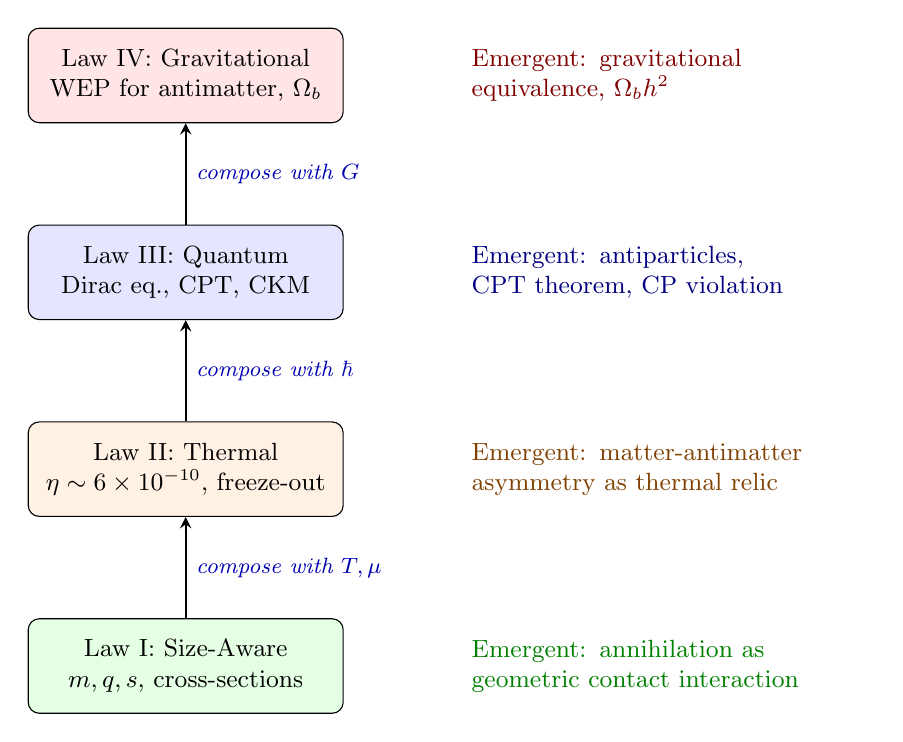
\begin{tikzpicture}[
    box/.style={rectangle, draw, rounded corners, minimum width=4cm, minimum height=1.2cm,
                align=center, font=\small},
    >=stealth
]
\node[box, fill=green!10] (L1) at (0,0) {Law I: Size-Aware\\$m, q, s$, cross-sections};
\node[box, fill=orange!10] (L2) at (0,2.5) {Law II: Thermal\\$\eta \sim 6 \times 10^{-10}$, freeze-out};
\node[box, fill=blue!10] (L3) at (0,5) {Law III: Quantum\\Dirac eq., CPT, CKM};
\node[box, fill=red!10] (L4) at (0,7.5) {Law IV: Gravitational\\WEP for antimatter, $\Omega_b$};

\draw[->, thick] (L1) -- (L2) node[midway, right, font=\footnotesize\itshape, text=blue!70!black] {compose with $T, \mu$};
\draw[->, thick] (L2) -- (L3) node[midway, right, font=\footnotesize\itshape, text=blue!70!black] {compose with $\hbar$};
\draw[->, thick] (L3) -- (L4) node[midway, right, font=\footnotesize\itshape, text=blue!70!black] {compose with $G$};

\node[right=1.5cm of L1, font=\small, text=green!50!black, text width=5cm, align=left] {Emergent: annihilation as\\geometric contact interaction};
\node[right=1.5cm of L2, font=\small, text=orange!50!black, text width=5cm, align=left] {Emergent: matter-antimatter\\asymmetry as thermal relic};
\node[right=1.5cm of L3, font=\small, text=blue!50!black, text width=5cm, align=left] {Emergent: antiparticles,\\CPT theorem, CP violation};
\node[right=1.5cm of L4, font=\small, text=red!50!black, text width=5cm, align=left] {Emergent: gravitational\\equivalence, $\Omega_b h^2$};
\end{tikzpicture}
\end{center}

%==============================================================================
\section{Experimental Detection and Current Results}
\label{sec:experiments}
%==============================================================================

\subsection{CERN Antimatter Factory}

The CERN Antiproton Decelerator (AD) and its successor, ELENA (Extra Low ENergy
Antiproton ring), provide low-energy antiprotons for precision measurements.
Several experiments operate at this facility:

\subsubsection{ALPHA Experiment}

The ALPHA (Antihydrogen Laser PHysics Apparatus) experiment traps antihydrogen
atoms ($\bar{p}e^+$) in a magnetic minimum trap and performs precision spectroscopy:

\begin{itemize}
    \item \textbf{1S--2S spectroscopy}: The $1S$--$2S$ two-photon transition frequency
    in antihydrogen has been measured to agree with hydrogen at the level of
    $2 \times 10^{-12}$~\cite{ALPHA2020}, providing a stringent CPT test.

    \item \textbf{ALPHA-g (2023)}: The first measurement of the gravitational acceleration
    of antimatter. Antihydrogen atoms released from the trap were observed to fall
    downward, confirming $\bar{g}/g = 1$ within $\sim 20\%$ uncertainty~\cite{ALPHA2023}.
    The experiment produced hundreds of antihydrogen atoms per experimental cycle.

    \item \textbf{Hyperfine structure}: The ground-state hyperfine splitting of
    antihydrogen has been measured and found consistent with hydrogen.
\end{itemize}

\subsubsection{BASE Experiment}

The BASE (Baryon Antibaryon Symmetry Experiment) uses single-particle Penning traps
to compare proton and antiproton properties with extreme precision:

\begin{itemize}
    \item \textbf{Charge-to-mass ratio}: The antiproton-to-proton charge-to-mass ratio
    has been measured to agree within 16 parts per trillion ($1.6 \times 10^{-11}$)~\cite{BASE2022}.

    \item \textbf{Magnetic moment}: The antiproton magnetic moment has been measured
    to $1.5$ parts per billion precision, agreeing with the proton value.
\end{itemize}

\subsubsection{AEgIS and GBAR Experiments}

AEgIS (Antimatter Experiment: Gravity, Interferometry, Spectroscopy) and GBAR
(Gravitational Behaviour of Antihydrogen at Rest) are dedicated experiments to
measure the gravitational acceleration of antihydrogen with increasing precision,
aiming for sub-percent-level tests of the weak equivalence principle for antimatter.

\subsection{LHCb: CP Violation Measurements}

The LHCb detector at the Large Hadron Collider is optimized for heavy-flavor physics
and CP violation measurements:

\begin{itemize}
    \item \textbf{2025 baryon CP violation}: First observation of CP violation in
    $\Lambda_b$ baryon decays~\cite{LHCb2025}, extending the CKM paradigm to the
    baryon sector.

    \item \textbf{CKM angle $\gamma$}: Most precise single-experiment measurement
    of the CKM angle $\gamma$ from tree-level $B^\pm \to DK^\pm$ decays.

    \item \textbf{$B_s$ mixing CP violation}: Measurements of CP violation in the
    $B_s$--$\bar{B}_s$ system, sensitive to new physics contributions.
\end{itemize}

\subsection{Cosmic Antimatter Searches}

\begin{itemize}
    \item \textbf{AMS-02}: The Alpha Magnetic Spectrometer on the International Space
    Station measures cosmic-ray positron and antiproton fluxes. The observed positron
    fraction excess above $\sim 10\GeV$ may indicate dark matter annihilation or
    pulsar contributions.

    \item \textbf{INTEGRAL}: The SPI spectrometer aboard INTEGRAL observes the
    511~keV annihilation line from the Galactic center, corresponding to $\sim 10^{43}$
    positron annihilations per second. The origin of these positrons remains debated
    (pulsars, dark matter, low-mass X-ray binaries).

    \item \textbf{Anti-nuclei searches}: AMS-02 has reported candidate anti-helium
    events, which if confirmed would have profound implications for cosmic antimatter
    domains or exotic production mechanisms.
\end{itemize}

%==============================================================================
\section{Applications of Anti-Matter}
\label{sec:applications}
%==============================================================================

\subsection{Positron Emission Tomography (PET)}

The most widespread practical application of antimatter is positron emission tomography,
a medical imaging technique:

\begin{definition}[PET Scanning Principle]
Positron emission tomography exploits positron--electron annihilation to produce
three-dimensional images of metabolic activity in living tissue.
\end{definition}

The physics chain is:
\begin{enumerate}
    \item A beta-plus ($\beta^+$) emitting radiopharmaceutical is administered
    (typically ${}^{18}\text{F}$-fluorodeoxyglucose, FDG, with $t_{1/2} = 109.77$ min).

    \item The nuclear decay $p \to n + e^+ + \nu_e$ produces a positron.

    \item The positron thermalizes within $\sim 1$~mm of the decay site and
    annihilates with an ambient electron:
    \begin{equation}
    e^+ + e^- \to \gamma + \gamma,
    \end{equation}
    producing two 511~keV photons emitted in nearly opposite directions (by
    momentum conservation).

    \item A ring of scintillation detectors records coincident photon pairs
    (within a $\sim 5$~ns timing window). The line connecting two coincident
    detectors passes through the annihilation point.

    \item Tomographic reconstruction (filtered back-projection or iterative algorithms)
    builds a 3D image of the radiotracer distribution.
\end{enumerate}

\begin{remark}
The 511~keV energy is precisely $m_e c^2 = 0.511\MeV$, a direct manifestation
of Einstein's mass--energy equivalence $E = mc^2$ applied to the complete conversion
of the electron--positron rest mass into photon energy.
\end{remark}

\subsection{Antiproton Cancer Therapy}

Antiproton beams have been investigated for cancer therapy, as antiproton annihilation
at the end of the beam range deposits additional energy (the annihilation products)
beyond the standard Bragg peak of proton therapy. The ACE experiment at CERN
demonstrated the feasibility, though clinical application remains distant due to
the difficulty and cost of producing antiproton beams.

\subsection{Antimatter Propulsion (Speculative)}

The energy density of matter--antimatter annihilation is the highest achievable:
$E = 2mc^2$ per annihilating pair, compared to $\sim 10^{-3} mc^2$ for nuclear fission
and $\sim 7 \times 10^{-3} mc^2$ for nuclear fusion. This has motivated speculative
proposals for antimatter-powered propulsion, though current production rates
($\sim 10^7$ antiprotons per second at CERN) make this impractical.

%==============================================================================
\section{Results: Collected Theorems and Formal Statements}
\label{sec:results}
%==============================================================================

We collect the main mathematical results established in this paper.

\begin{theorem}[Master Theorem: Anti-Matter as Modular Emergence]
\label{thm:master}
In the modular physics framework, anti-matter and the matter--antimatter asymmetry
arise through the following chain of modular compositions:

\begin{enumerate}
    \item \textbf{Quantum $\circ$ Lorentz $\Rightarrow$ Anti-matter}:
    The composition of quantum mechanics with Lorentz invariance (Law~III)
    necessarily produces antiparticles (\cref{thm:emergent_antimatter}).

    \item \textbf{Locality $\circ$ Lorentz $\circ$ Unitarity $\Rightarrow$ CPT}:
    The composition of locality, Lorentz invariance, and unitarity produces CPT
    invariance as an emergent symmetry (\cref{thm:cpt}).

    \item \textbf{Three Generations $\circ$ Unitarity $\Rightarrow$ CP Violation}:
    The composition of three quark generations with the unitarity of the CKM matrix
    produces exactly one irremovable CP-violating phase (\cref{thm:three_gen}).

    \item \textbf{CP Violation $\circ$ Thermal $\circ$ B Violation $\Rightarrow$ Baryogenesis}:
    The composition of CP violation with thermal physics and baryon number violation
    produces the matter--antimatter asymmetry (\cref{thm:sakharov}).

    \item \textbf{Baryogenesis $\circ$ Gravity $\Rightarrow$ $\Omega_b$}:
    The baryon asymmetry, when composed with gravitational dynamics, determines the
    baryonic matter content of the universe (\cref{thm:hierarchical_cp}).
\end{enumerate}
Each arrow represents a modular composition producing emergent properties absent
from either ingredient alone.
\end{theorem}

\begin{lemma}[Quantitative Insufficiency of CKM CP Violation]
\label{lem:ckm_insufficient}
The baryon asymmetry produced by Standard Model electroweak baryogenesis, using only
the CKM source of CP violation, satisfies:
\begin{equation}
\eta_{\text{SM}} \lesssim 10^{-20} \ll \eta_{\text{obs}} \approx 6 \times 10^{-10}.
\end{equation}
\end{lemma}

\begin{proof}[Proof sketch]
The baryon asymmetry from EWBG scales as~\cite{ShaposhnikovReview}:
\begin{equation}
\eta \sim \frac{n_B}{s} \sim \frac{g^2}{T^3} \cdot \frac{\Gamma_{\text{sph}}}{H} \cdot \delta_{\text{CP}} \cdot \kappa,
\end{equation}
where $\Gamma_{\text{sph}}/H$ is the sphaleron rate relative to the Hubble rate,
$\delta_{\text{CP}}$ encodes the CP-violating source, and $\kappa$ is an efficiency
factor. In the Standard Model:
\begin{itemize}
    \item The Jarlskog invariant $J \sim 10^{-5}$ suppresses $\delta_{\text{CP}}$.
    \item An additional suppression by the quark mass hierarchy
    $\prod_{i<j}(m_{u_i}^2 - m_{u_j}^2)(m_{d_i}^2 - m_{d_j}^2)/v^{12}$ further
    reduces the effective CP violation.
    \item The electroweak phase transition is a crossover (not first-order) for
    $m_H = 125\GeV$, giving $\kappa \approx 0$.
\end{itemize}
The combined effect yields $\eta_{\text{SM}} \lesssim 10^{-20}$.
\end{proof}

\begin{corollary}[Necessity of Beyond-Standard-Model Physics]
\label{cor:bsm}
The observed baryon asymmetry $\eta \approx 6 \times 10^{-10}$ requires at least one
of the following extensions beyond the Standard Model:
\begin{enumerate}
    \item Additional sources of CP violation (new complex phases in the scalar,
    neutrino, or dark sector).
    \item A first-order electroweak phase transition (from extended Higgs sectors,
    singlet scalars, or composite Higgs models).
    \item New baryogenesis mechanisms at higher energy scales (leptogenesis,
    GUT baryogenesis, Affleck--Dine).
\end{enumerate}
\end{corollary}

\begin{proposition}[Quantitative CPT Tests]
\label{prop:cpt_tests}
The current experimental bounds on CPT violation, expressed as relative differences,
are:
\begin{center}
\begin{tabular}{lcc}
\hline
Observable & Bound & Experiment \\
\hline
$|m_{K^0} - m_{\bar{K}^0}|/m_K$ & $< 6 \times 10^{-19}$ & CPLEAR \\
$|q/m|_{\bar{p}} / |q/m|_p - 1$ & $< 1.6 \times 10^{-11}$ & BASE \\
$|g_e - g_{\bar{e}}|/g_e$ & $< 2 \times 10^{-12}$ & Harvard \\
$|\nu_{1S-2S}^{\bar{H}} - \nu_{1S-2S}^{H}|/\nu$ & $< 2 \times 10^{-12}$ & ALPHA \\
\hline
\end{tabular}
\end{center}
All are consistent with exact CPT invariance.
\end{proposition}

%==============================================================================
\section{Discussion}
\label{sec:discussion}
%==============================================================================

\subsection{Interpretive Significance of the Modular Framework}

The modular physics framework provides a natural organizational principle for
understanding anti-matter. Rather than treating anti-matter as a separate ``substance,''
the framework reveals it as an emergent consequence of the composition of fundamental
laws:

\begin{enumerate}
    \item Anti-matter is \emph{not} a new ingredient added to the theory; it emerges
    automatically from the requirement of consistency (Lorentz invariance + quantum mechanics).
    This is the hallmark of genuine emergence in the modular framework: the composed
    system has properties that neither component possesses individually.

    \item The CPT theorem is similarly emergent: it is not postulated but derived
    from the compositional axioms (locality, Lorentz invariance, unitarity).

    \item CP violation requires a specific compositional structure: three generations
    of quarks with a unitary mixing matrix. Two generations are insufficient.
    This is a topological fact about the parameter space of unitary matrices.

    \item The matter--antimatter asymmetry is a thermal relic that requires the
    composition of quantum CP violation with thermodynamic non-equilibrium
    (Sakharov's conditions). Neither ingredient alone produces the asymmetry.
\end{enumerate}

\subsection{The Baryogenesis Problem as a Modular Gap}

The failure of Standard Model EWBG to produce the observed baryon asymmetry
identifies a \emph{modular gap}: the known composition of Law~II (Thermal) with
Law~III (Quantum, specifically the CKM mechanism) is quantitatively insufficient.
This gap points to one of two resolutions:

\begin{itemize}
    \item \textbf{New physics at Law~III}: Additional CP-violating sectors (neutrino
    Majorana phases, dark sector CP violation, extended Higgs sector) that compose
    with Law~II to produce a sufficient asymmetry.

    \item \textbf{New physics at the Law~III--IV interface}: The baryogenesis mechanism
    may involve gravitational or trans-Planckian physics, such as gravitational
    leptogenesis or baryogenesis during inflation.
\end{itemize}

\subsection{Open Problems}

\begin{enumerate}
    \item \textbf{The baryogenesis problem}: What is the dynamical mechanism that
    produced $\eta \approx 6 \times 10^{-10}$? This remains the central open question
    in anti-matter physics.

    \item \textbf{New sources of CP violation}: The CKM phase is insufficient. Where
    is the additional CP violation? Candidates include the PMNS matrix (leptonic CP phase
    $\delta_{\text{CP}}$), strong CP ($\theta_{\text{QCD}}$), and beyond-Standard-Model sectors.

    \item \textbf{Majorana neutrinos}: Are neutrinos their own antiparticles? If so,
    the distinction between matter and anti-matter is blurred in the lepton sector.
    Neutrinoless double-beta decay searches (GERDA, CUORE, KamLAND-Zen, nEXO) probe
    this question.

    \item \textbf{Antimatter gravity}: The ALPHA-g result confirms antimatter falls
    downward but with $\sim 20\%$ precision. Future experiments (AEgIS, GBAR) aim for
    sub-percent precision tests of the weak equivalence principle.

    \item \textbf{Cosmic antimatter domains}: While largely ruled out by CMB isotropy
    arguments, the possibility of antimatter domains separated from matter domains at
    cosmological scales has not been definitively excluded. Anti-helium candidates
    in AMS-02 data could provide evidence.

    \item \textbf{Strong CP problem}: Why is $\theta_{\text{QCD}} \leq 10^{-10}$?
    The Peccei--Quinn mechanism predicts the axion, which would also be a dark matter
    candidate.

    \item \textbf{Absolute neutrino mass scale}: KATRIN constrains $m_\nu < 0.45\text{ eV}$
    (90\% CL, 2024). The absolute mass scale affects leptogenesis models.
\end{enumerate}

\subsection{Connections to Other Standard Model Topics}

Anti-matter connects to virtually every sector of the Standard Model:
\begin{itemize}
    \item \textbf{Quark model}: Every quark has an antiquark; mesons are $q\bar{q}$ states.
    \item \textbf{QCD}: Color confinement applies equally to quarks and antiquarks;
    color charge conjugation maps $\mathbf{3} \to \bar{\mathbf{3}}$.
    \item \textbf{Electroweak theory}: The $W^\pm$ bosons mediate transitions between
    quarks and antiquarks; the CKM matrix governs flavor-changing charged currents.
    \item \textbf{Higgs mechanism}: The Yukawa couplings that give fermion masses
    simultaneously determine the CKM matrix through the mismatch between up-type
    and down-type Yukawa matrices.
    \item \textbf{Neutrino physics}: The PMNS matrix is the leptonic analogue of the
    CKM matrix, potentially containing additional CP-violating phases relevant to
    leptogenesis.
\end{itemize}

%==============================================================================
\section{Conclusion}
\label{sec:conclusion}
%==============================================================================

We have presented a comprehensive treatment of anti-matter within the modular physics
framework, demonstrating that:

\begin{enumerate}
    \item Anti-matter emerges as a necessary consequence of the modular composition
    of quantum mechanics with special relativity (Law~III), through the Dirac equation
    and the Feynman--St\"uckelberg interpretation of negative-energy solutions.

    \item The CPT theorem---guaranteeing exact particle--antiparticle symmetry in
    masses, lifetimes, and (magnitude of) magnetic moments---is an emergent property
    of the compositional axioms: Lorentz invariance, locality, unitarity, and the
    spin-statistics connection.

    \item CP violation in the Standard Model arises from the single irremovable phase
    in the $3 \times 3$ CKM matrix, requiring exactly three generations of quarks.
    The 2025 LHCb observation of CP violation in baryon decays extends the
    Kobayashi--Maskawa paradigm to the baryon sector.

    \item The matter--antimatter asymmetry ($\eta \approx 6 \times 10^{-10}$) requires
    all three Sakharov conditions, representing a composition of quantum CP violation
    with thermal non-equilibrium dynamics and baryon number violation.

    \item The Standard Model CKM mechanism is quantitatively insufficient for
    baryogenesis by at least ten orders of magnitude, identifying a modular gap
    that points toward physics beyond the Standard Model.

    \item Experimental tests at CERN (ALPHA, BASE, AEgIS) confirm CPT invariance
    at extraordinary precision and have provided the first measurement of antimatter's
    gravitational behavior, consistent with the weak equivalence principle.
\end{enumerate}

The modular framework reveals anti-matter not as an exotic addendum to physics but as
the inevitable consequence of compositional structure: each level of the hierarchy
(Size-Aware $\to$ Thermal $\to$ Quantum $\to$ Gravitational) produces emergent
phenomena---from antiparticles themselves, to the CPT theorem, to the baryon
asymmetry---that are invisible at lower compositional levels. The baryogenesis
problem stands as the most compelling evidence that our current modular composition
is incomplete and that new physics awaits discovery.

%==============================================================================
% References
%==============================================================================
\begin{thebibliography}{99}

\bibitem{Dirac1928}
P.~A.~M.~Dirac, ``The quantum theory of the electron,''
\textit{Proc.\ R.\ Soc.\ Lond.\ A} \textbf{117}, 610--624 (1928).

\bibitem{Dirac1930}
P.~A.~M.~Dirac, ``A theory of electrons and protons,''
\textit{Proc.\ R.\ Soc.\ Lond.\ A} \textbf{126}, 360--365 (1930).

\bibitem{Anderson1933}
C.~D.~Anderson, ``The positive electron,''
\textit{Phys.\ Rev.} \textbf{43}, 491--494 (1933).

\bibitem{Wu1957}
C.~S.~Wu \textit{et al.}, ``Experimental test of parity conservation in beta decay,''
\textit{Phys.\ Rev.} \textbf{105}, 1413--1415 (1957).

\bibitem{CroninFitch1964}
J.~H.~Christenson, J.~W.~Cronin, V.~L.~Fitch, and R.~Turlay,
``Evidence for the $2\pi$ decay of the $K_2^0$ meson,''
\textit{Phys.\ Rev.\ Lett.} \textbf{13}, 138--140 (1964).

\bibitem{Cabibbo1963}
N.~Cabibbo, ``Unitary symmetry and leptonic decays,''
\textit{Phys.\ Rev.\ Lett.} \textbf{10}, 531--533 (1963).

\bibitem{KobayashiMaskawa1973}
M.~Kobayashi and T.~Maskawa, ``CP-violation in the renormalizable theory of weak interaction,''
\textit{Prog.\ Theor.\ Phys.} \textbf{49}, 652--657 (1973).

\bibitem{Sakharov1967}
A.~D.~Sakharov, ``Violation of CP invariance, C asymmetry, and baryon asymmetry of the universe,''
\textit{JETP Lett.} \textbf{5}, 24--27 (1967).

\bibitem{StreaterWightman}
R.~F.~Streater and A.~S.~Wightman,
\textit{PCT, Spin and Statistics, and All That},
Princeton University Press (1964, reprinted 2000).

\bibitem{Weinberg1995}
S.~Weinberg, \textit{The Quantum Theory of Fields}, Vol.~1,
Cambridge University Press (1995).

\bibitem{CPLEAR1998}
CPLEAR Collaboration, ``First direct observation of time-reversal non-invariance
in the neutral-kaon system,''
\textit{Phys.\ Lett.\ B} \textbf{444}, 43--51 (1998).

\bibitem{BaBar2001}
BaBar Collaboration, ``Observation of CP violation in the $B^0$ meson system,''
\textit{Phys.\ Rev.\ Lett.} \textbf{87}, 091801 (2001).

\bibitem{Belle2001}
Belle Collaboration, ``Observation of large CP violation in the neutral $B$ meson system,''
\textit{Phys.\ Rev.\ Lett.} \textbf{87}, 091802 (2001).

\bibitem{BaBar2012}
BaBar Collaboration, ``Observation of time-reversal violation in the $B^0$ meson system,''
\textit{Phys.\ Rev.\ Lett.} \textbf{109}, 211801 (2012).

\bibitem{LHCb2025}
LHCb Collaboration, ``Observation of CP violation in baryon decays,''
\textit{Nature} (2025), \texttt{doi:10.1038/s41586-025-09119-3}.

\bibitem{ALPHA2020}
ALPHA Collaboration, ``Investigation of the fine structure of antihydrogen,''
\textit{Nature} \textbf{578}, 375--380 (2020).

\bibitem{ALPHA2023}
ALPHA Collaboration, ``Observation of the effect of gravity on the motion of antimatter,''
\textit{Nature} \textbf{621}, 716--722 (2023).

\bibitem{BASE2022}
BASE Collaboration, ``A 16-parts-per-trillion measurement of the antiproton-to-proton
charge-to-mass ratio,'' \textit{Nature} \textbf{601}, 53--57 (2022).

\bibitem{Hanneke2008}
D.~Hanneke, S.~Fogwell, and G.~Gabrielse,
``New measurement of the electron magnetic moment and the fine structure constant,''
\textit{Phys.\ Rev.\ Lett.} \textbf{100}, 120801 (2008).

\bibitem{PDG2024}
Particle Data Group, R.~L.~Workman \textit{et al.},
``Review of Particle Physics,''
\textit{Prog.\ Theor.\ Exp.\ Phys.} \textbf{2024}, 083C01 (2024).

\bibitem{Planck2018}
Planck Collaboration, ``Planck 2018 results. VI. Cosmological parameters,''
\textit{Astron.\ Astrophys.} \textbf{641}, A6 (2020).

\bibitem{DavidsonIbarra2002}
S.~Davidson and A.~Ibarra, ``A lower bound on the right-handed neutrino mass from
leptogenesis,'' \textit{Phys.\ Lett.\ B} \textbf{535}, 25--32 (2002).

\bibitem{ShaposhnikovReview}
M.~Shaposhnikov, ``Baryogenesis,''
\textit{J.\ Phys.\ Conf.\ Ser.} \textbf{171}, 012005 (2009).

\bibitem{ConversionDriven2024}
A.~Granelli \textit{et al.}, ``Conversion-driven leptogenesis,''
\textit{Phys.\ Rev.\ Lett.} \textbf{133}, 191803 (2024).

\bibitem{SupercooledConfinement2024}
I.~Baldes \textit{et al.}, ``Baryogenesis from supercooled confinement,''
\textit{JHEP} \textbf{2024}, 063 (2024).

\bibitem{LudersPauli1954}
G.~L\"uders, ``On the equivalence of invariance under time reversal and under
particle-antiparticle conjugation for relativistic field theories,''
\textit{Dansk.\ Mat.\ Fys.\ Medd.} \textbf{28}, no.~5, 1--17 (1954).

\bibitem{Schwinger1951}
J.~Schwinger, ``The theory of quantized fields. I,''
\textit{Phys.\ Rev.} \textbf{82}, 914--927 (1951).

\bibitem{Jost1957}
R.~Jost, ``A remark on the C.T.P. theorem,''
\textit{Helv.\ Phys.\ Acta} \textbf{30}, 409--416 (1957).

\end{thebibliography}

\end{document}
